\chapter{Project Plan}

\instructions{
    Describe the project plan as covered in the SEP2 module. A project plan typically consists of the following topics:
    
    \begin{itemize}
        \item Processes, meetings and roles
        \item Phases, iterations and milestones
        \item A \textbf{rough} list of things to be done (work items)
        \item Risk management
        \item Planning Tools (issue tracker, time tracker, ...)
    \end{itemize}
    
    You should \textbf{\underline{not}} describe your \textbf{technical solution} in this chapter. It is all about organizing your project.
}

\section{Relevant Links}

The following chapters are referencing external tools. For convenience, those tools are also listed here:

\begin{itemize}
    \item GitLab: \url{https://gitlab.ost.ch/SEProj/2022-FS/g02-jasstracker/jasstracker}
    \item Jira: \url{https://jasstracker-jira.atlassian.net/browse/JASS}
\end{itemize}

\section{Processes}

We will use a combination of Scrum (without RUP) because all team members are comfortable with Scrum.
Milestones, iterations and epics are tracked in Jira (see \ref{sec:TimeAndIssueTracking}).

\subsection*{Meetings}

\begin{table}[H]
    \begin{tabular}{l|l|l|l}
    \textbf{Meeting} & \textbf{Schedule} & \textbf{Subject} & \textbf{Timebox} \\
    \hline
    Weekly & Every Saturday & Scrum Daily & 15m \\
    Planning & Every other Tuesday & Scrum Planning & 45m \\
    Retro & Every other Tuesday & Scrum Retrospective & 45m \\
    Review 1 & 07.03.2022 & Project Plan & 1h \\
    Review 2 & 21.03.2022 & Requirements & 1h \\
    Review 3 & 04.04.2022 & End of Elaboration & 1h \\
    Review 4 & 02.05.2022 & Quality & 1h \\
    Review 5 & 23.05.2022 & Architecture & 1h \\
    Presentation & 07.06.2022 & Present the great JassTracker & 1h
    \end{tabular}
\end{table}

\subsection*{Roles}

Because of the small team size some members have more than one assigned role.

\begin{table}[H]
    \begin{tabular}{l|l|l}
    \textbf{Who} & \textbf{Roles} & \textbf{Responsibilities} \\
    \hline
    Pascal & PO, DEV & Push project vision, provide business feedback \\
    Marcel & DEVOPS & Setup and maintain operations, continous delivery \\
    David  & SM, DEV & Ensure correct scrum procedure \\
    Jamie  & QA, DEV & Guarantee the final product has a good quality and works reliably
    \end{tabular}
\end{table}

\subsubsection*{DEV}
A developer is responsible for the development of the target application.
Every developer is responsible for the project / code quality as a whole and should act accordingly.

\subsubsection*{PO}
The product owner is responsible to push the project vision forward.
In planning meetings, he is responsible to get as many features done as possible.
The product backlog is mainly created by the PO, but the team as a whole is responsible for maintaining it.
But the PO has full authority over the priorization of user stories.

\subsubsection*{DEVOPS}
A devops engineer extends all responsibilities from a regular dev.
In addition, he is responsible for operating the app by ensuring it's working correctly.
He manages and oversees the deployment process and tracks metrics such as uptime or hardware utilization.

\subsubsection*{SM}
The scrum master is responsible for the correct implementation of the scrum process.
He is in charge of organizing the scrum meetings and document them if needed (e.g. Retrospective)

\subsubsection*{QA}
Quality Assurance is responsible to ensure a good quality of the final product.
To achieve this, quality metrics should be setup and tracked by QA, such as test coverage.
It is not in the responsibility of QA to fix such issues or run manual tests, that honor belongs to the whole team.

\section{Collaboration}

We're using MS Teams for internal communication.
We plan on using the \href{https://gitlab.ost.ch/SEProj/2022-FS/g02-jasstracker/jasstracker}{OST GitLab} for version control.
Changes are always done on seperate branches and integrated through merge requests with a required code review.

\section{Risk Management}

\subsection{Very High}
\begin{enumerate}
    \item Used technologies are not well knows by all team members (certain, critical) 
    \begin{enumerate}
        \item Mitigation: Every team member should create a PoC in the used technologies to ensure basic understanding is present 
    \end{enumerate}
\end{enumerate}

\subsection{High}
\begin{enumerate}
    \item Inaccurate estimations (likely and critical) 
    \begin{enumerate}
        \item Mitigation strategies: apply cone of uncertainty, apply definion of ready to ensure planning quality 
    \end{enumerate}

    \item Poor risk management (likely and critical)  
    \begin{enumerate}
        \item Mitigation strategies: likelihood calculation, risk mitigation plans and monitoring of risks every planning 
    \end{enumerate}

    \item Project reviewer's expectations are not aligned with project (possible and critical) 
    \begin{enumerate}
        \item Mitigation strategies: obtain frequent approval and acknowledgement (naturally happens for us with review meetings) 
    \end{enumerate}

    \item Unexpected absence of team member (unlikely and catastrophic) 
    \begin{enumerate}
        \item Mitigation strategies: Code changes need to be pushed on a daily basis, stories could at any point be taken over by another team member 
    \end{enumerate}
\end{enumerate}

\subsection{Medium}
\begin{enumerate}
    \item Insufficient code quality (possible and marginal) 
    \begin{enumerate}
        \item Mitigation strategies: code reviews, clear coding standards, apply definition of done 
    \end{enumerate}

    \item Lack of ownership (possible and marginal) 
    \begin{enumerate}
        \item Mitigation strategies: setting clear responsibilities for roles 
    \end{enumerate}

    \item Losing sight of documentation tasks (possible and marginal) 
    \begin{enumerate}
        \item Mitigation strategies: documentation strategy , documentation part of definiton of done 
    \end{enumerate}

    \item Failure of hardware like personal devices, OST GitLab, Jira, hosted environment (rare, catastrophic) 
    \begin{enumerate}
        \item Mitigation strategies: Code changes need to be pushed on a daily basis 
    \end{enumerate}
\end{enumerate}

\subsection{Low}
\begin{enumerate}
    \item Project idea, "Jassen", is not well known or understood by team members (possible, negligible) 
    \begin{enumerate}
        \item Mitigation strategies:  Play a "Jass" in the team to ensure everybody knows the basic rules and concepts 
    \end{enumerate}
\end{enumerate}

\section{Time \& Issue Tracking} \label{sec:TimeAndIssueTracking}

Our project plan is tracked on our \href{https://jasstracker-jira.atlassian.net/browse/JASS}{Jira Board}.
All team members are already experienced with Jira and it provides many desired features (Epics, burndown charts, sprints) which were lacking in GitLab.

\subsection{Roadmap}
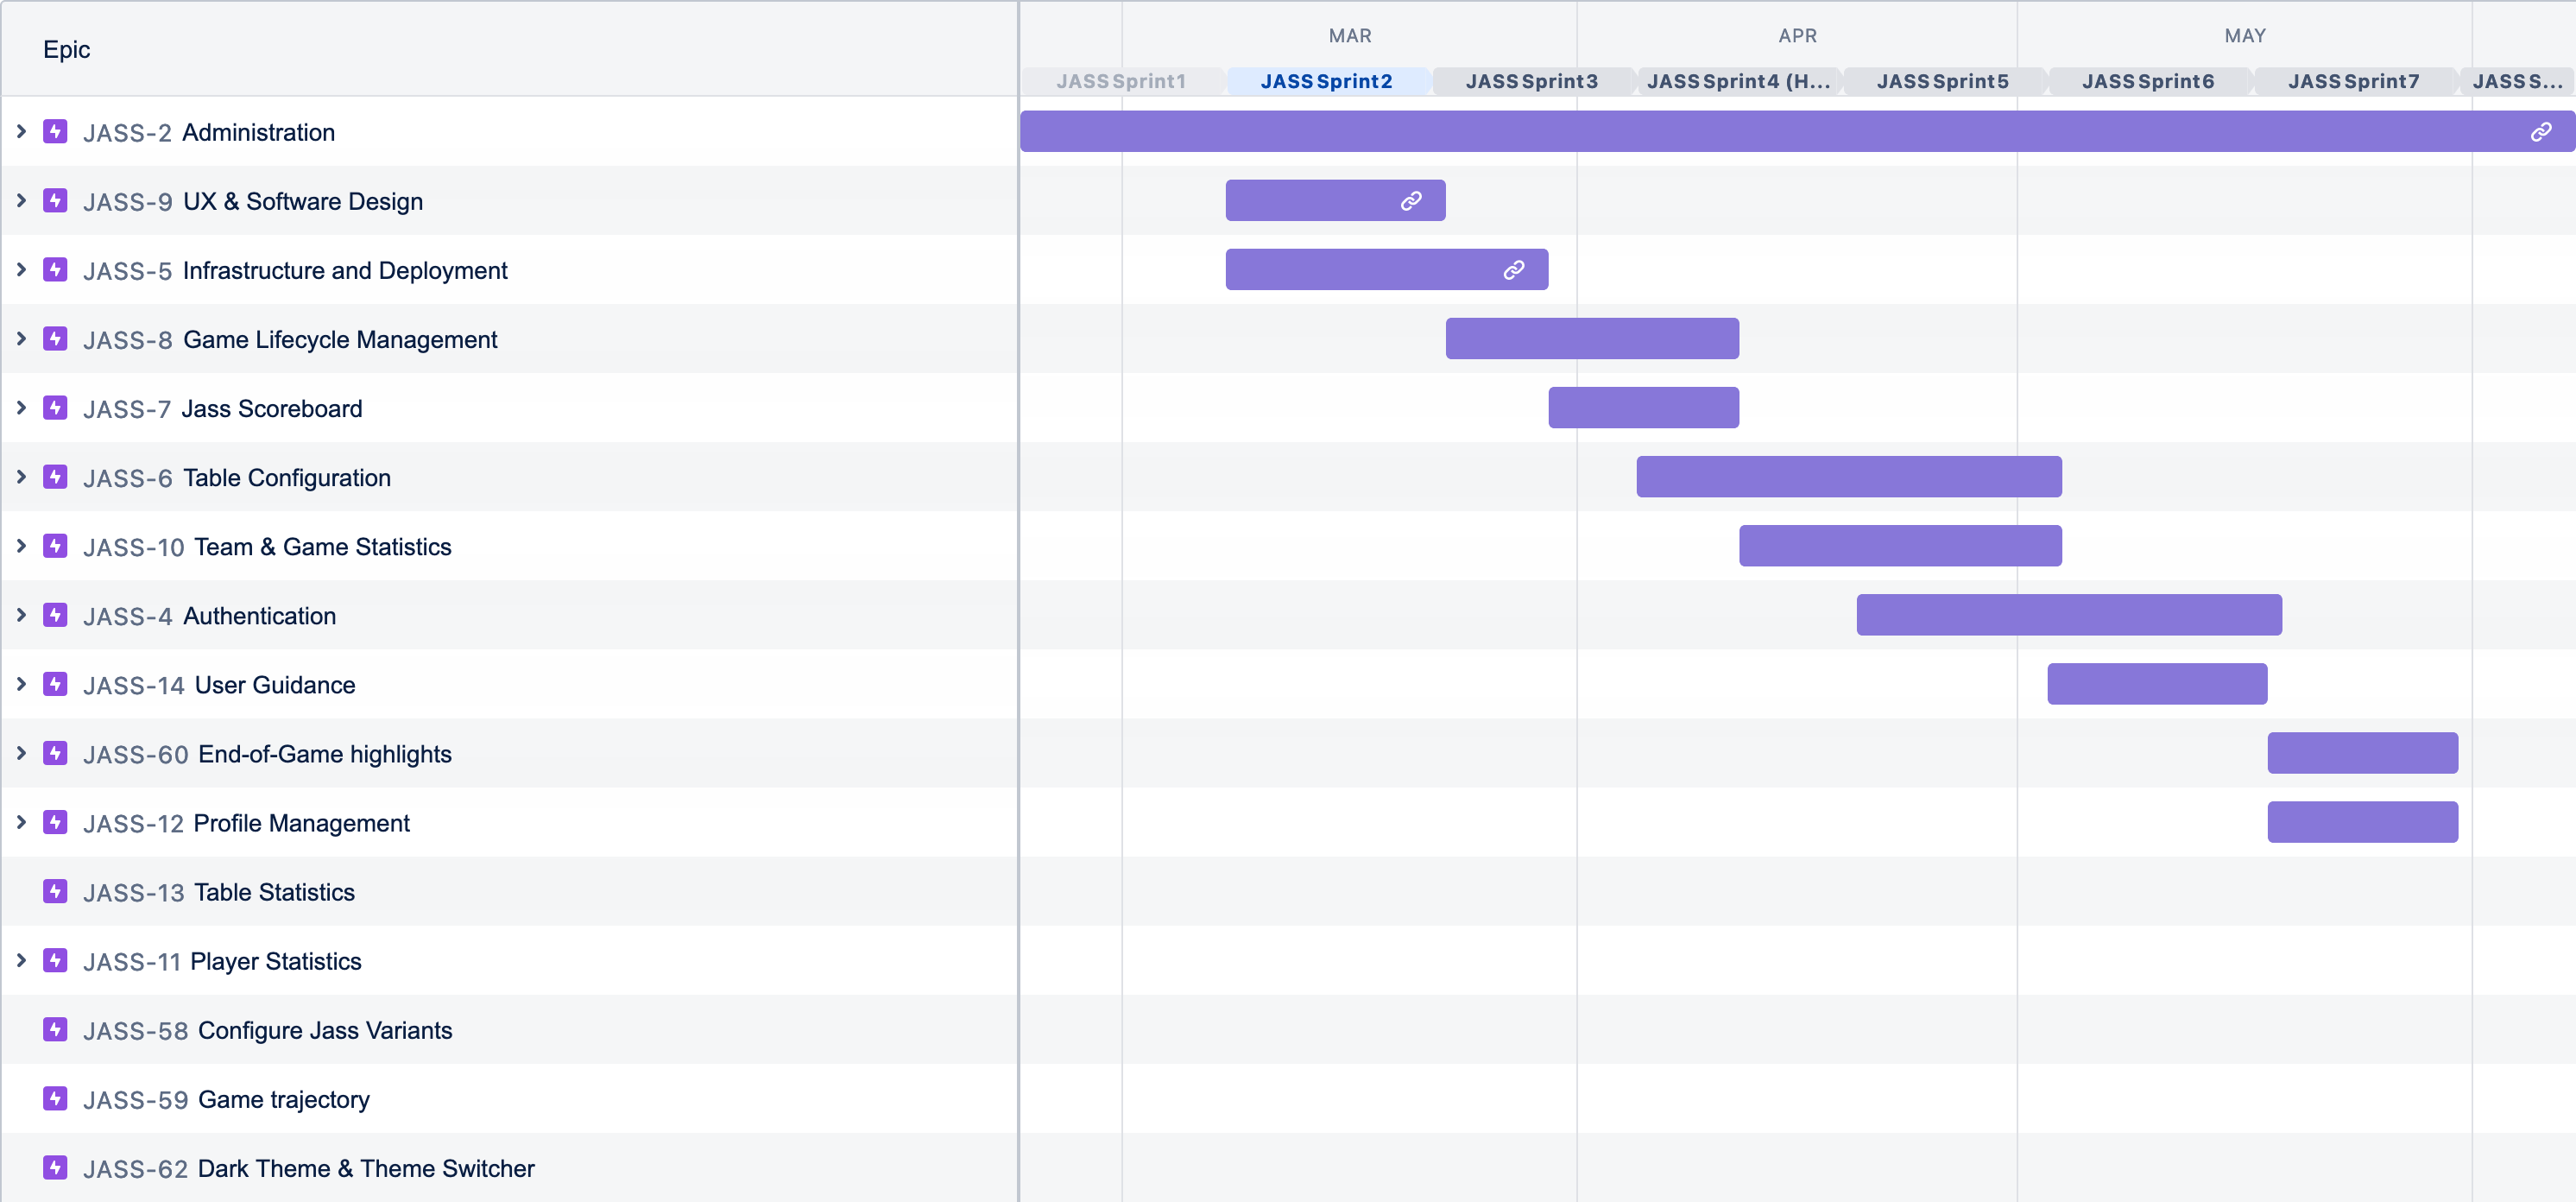
\includegraphics[width=\textwidth]{resources/jira-roadmap.png}